\chapter{Analysis with MG-MAMPOSSt code}\label{Capitolo4}

Modify Gravity -- Modelling Anisotropy and Mass Profiles of Observed Spherical Systems\footnote{In this thesis we are not interested with modify gravity, so the code is used under General Relativity regime.} (or \textsc{MG-MAMPOSSt} hereafter) is a program that derives the mass profile of galaxy clusters from the analysis of the kinematics of galaxies with the hypothesis that the system has spherical symmetry and dynamical relaxation. It's the evolution of the previous method \textsc{MAMPOSSt} (ref. \cite{Biviano_MAMPOSSt}), able to work in standard gravity as well as in many non-standard scenarios including popular dark energy/modified gravity frameworks (see ref. \cite{pizzuti2022mgmamposstcodetestgravity}).\\ 
The code explores the projected phase space composed of the projected position of the galaxy and velocity along the line of sight indicated with $v_z$ and called l.o.s. hereafter. These speeds refer to the cluster rest frame.\\
To determine the velocities along the line of sight, redshift data, which in turn are obtained from spectroscopic analyses, is used as described in the end of the previous chapter. The velocities are assumed to be distributed according to a Gaussian.
\textsc{MG-MAMPOSSt} also attributes a parametric profile characterized by velocity anisotropy, gravitational potential, mass profile and number density profile. Then, Jeans's equation \eqref{Equazione di Jeans sferica}, under the assumption of dynamic equilibrium and spherical symmetry, is resolved and likelihoods are computed over a multidimensional grid of values. In order to do this, the code uses a Monte Carlo Markov Chain (or MCMC) which is particularly useful for a large number of parameters or a large number of haloes.\\ 
\textsc{MG-MAMPOSSt} can use different types of priors: flat and Gaussian. Flat priors can be used in case you do not want to privilege any particular value within a given range. Conversely, a Gaussian prior is a prior that assumes that the parameter is distributed around a preferred central value with some standard deviation. 
The final results are a series of posteriors found and $- \log(\mathcal{L})$.\\
In figure \ref{Flux diagram MG-MAMPOSSt}, the steps performed by the code are outlined and summarized.
\begin{figure}
    \centering
    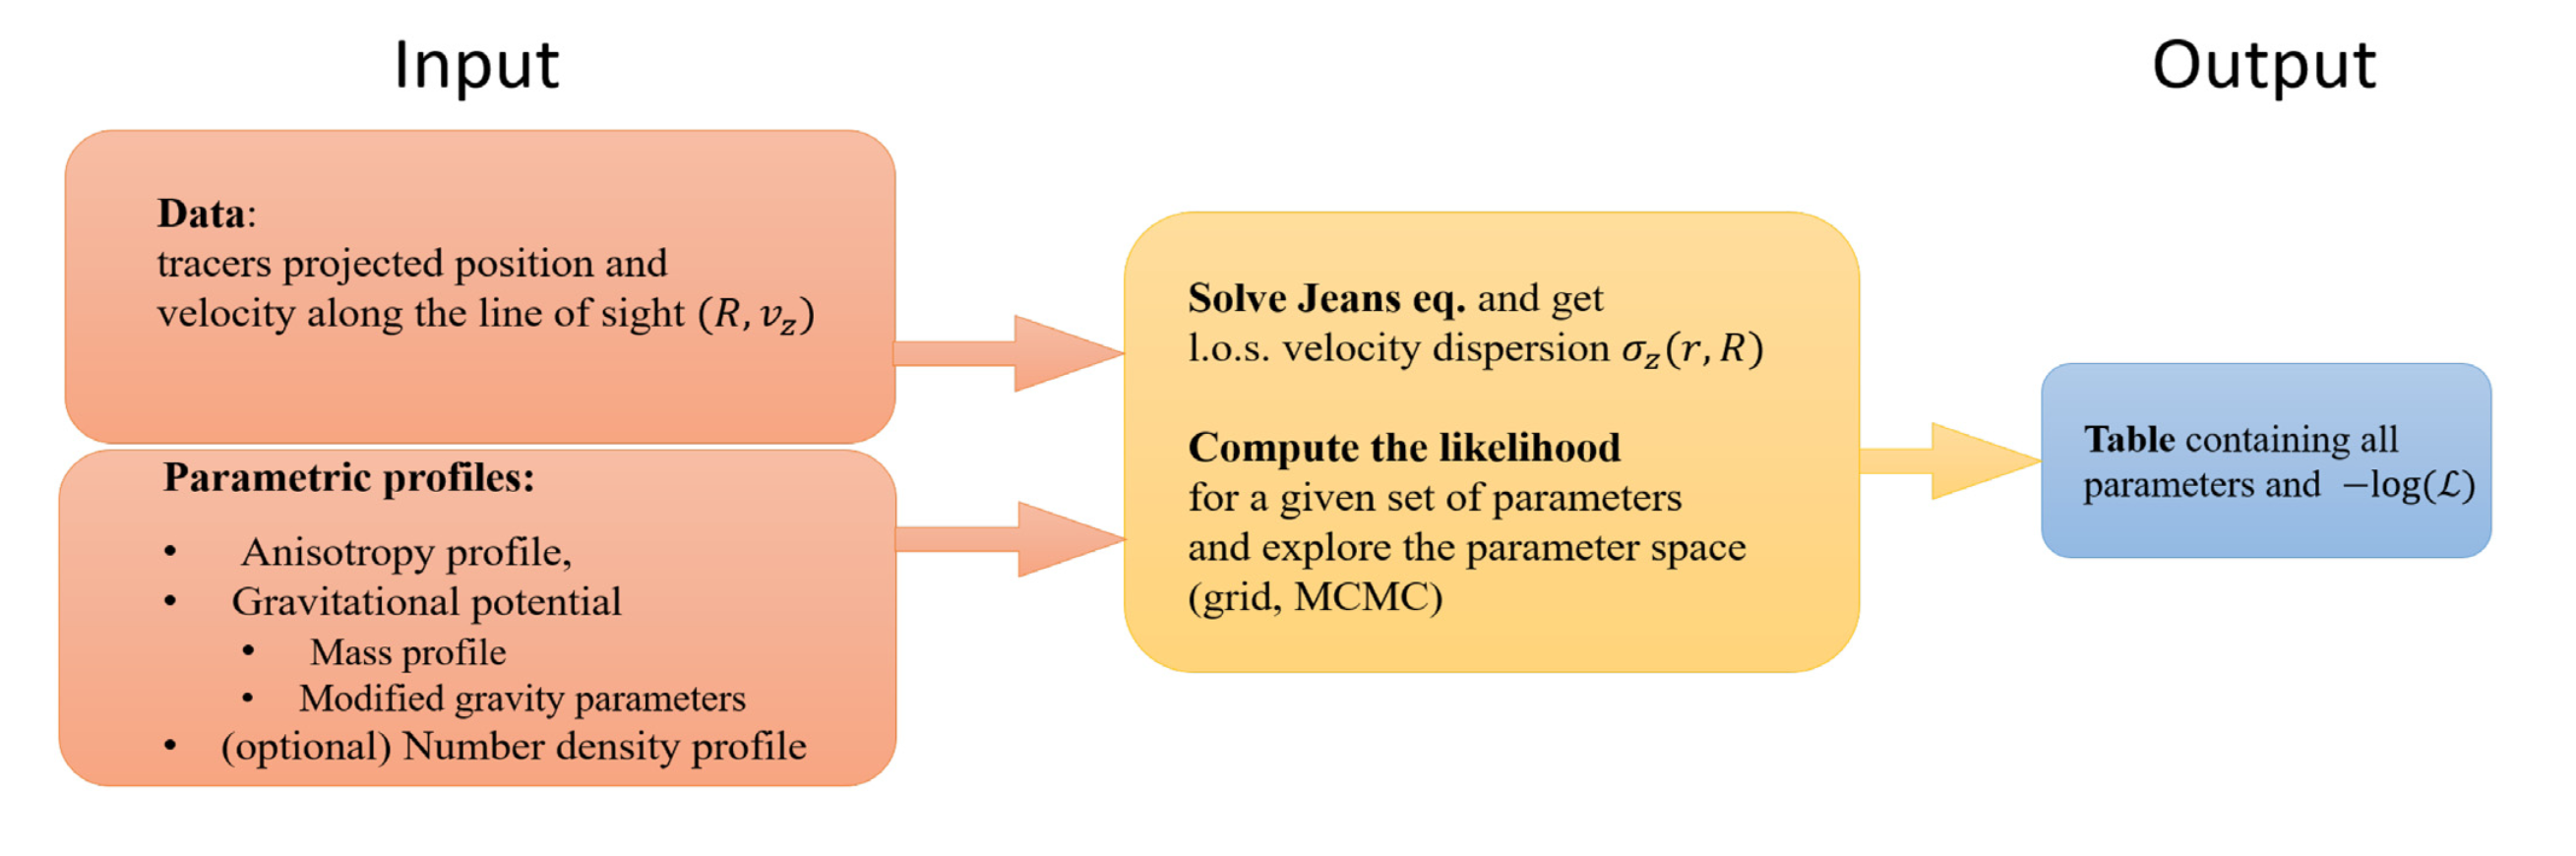
\includegraphics[width=0.99\linewidth]{Images/Chapter4/Flux diagram MG-MAMPOSSt.png}
    \caption[Flux diagram \textsc{MG-MAMPOSSt}]{Flux diagram \textsc{
    MG-MAMPOSSt}. Figure 1 in ref. \cite{MG-MAMPOSST:a-code-to-test-modifications-of-gravity-with-internal-kinematics-and-lensing-analyses-of-galaxy-clusters}.}
    \label{Flux diagram MG-MAMPOSSt}
\end{figure}

It's important to notice that the anisotropy profile is not known at the beginning. For this reason, many models are available\footnote{See ref. \cite{pizzuti2022mgmamposstcodetestgravity} to explore all models in \textsc{MG-MAMPOSSt.}}, but in this thesis, two models are adopted: generalized Tiret model, indicated gT (see e.g. ref. \cite{Mamon_2019}), and Biviano$\&$Pizzuti model (BP). Generalized Tiret profile has the following functional form:
\begin{equation} \label{gT model}
    \beta_{gT}(r) = \beta_0 + (\beta_\infty - \beta_0) \frac{r}{r + r_\beta},
\end{equation}
where $\beta_0$ is the anisotropy in the center of the cluster and $\beta_\infty$ is the anisotropy for $r\to\infty$, with transition radius fixed by $r_\beta$ (ref. \cite{pizzuti2022mgmamposstcodetestgravity}). While the BP profile presents the following analytical distribution
\begin{equation} \label{BP model}
    \beta(r) = \beta_0 + (\beta_\infty - \beta_0) \frac{r}{r+r_\beta} + \beta_\infty \frac{r^2}{r^2 _\beta} \exp \qty[-\qty(\frac{r}{r_\beta})^2].
\end{equation}
As for the number density profile of the galaxies, we will always assume a NFW model. This choice is not causal, but based on ref. \cite{CLASH-VLT:-The-Inner-Slope-of-the-MACS-J1206.2-0847-Dark-Matter-Density-Profile}, where the spectroscopic data were corrected to compensate for the incompleteness at different clustercentric radii due to the different depths with which VIMOS and MUSE observed galaxies. After the correction, projected NFW proves suitable for fitting the number density of galaxies. This is clearly visible in the following plot.
\begin{figure}[h!]
    \centering
    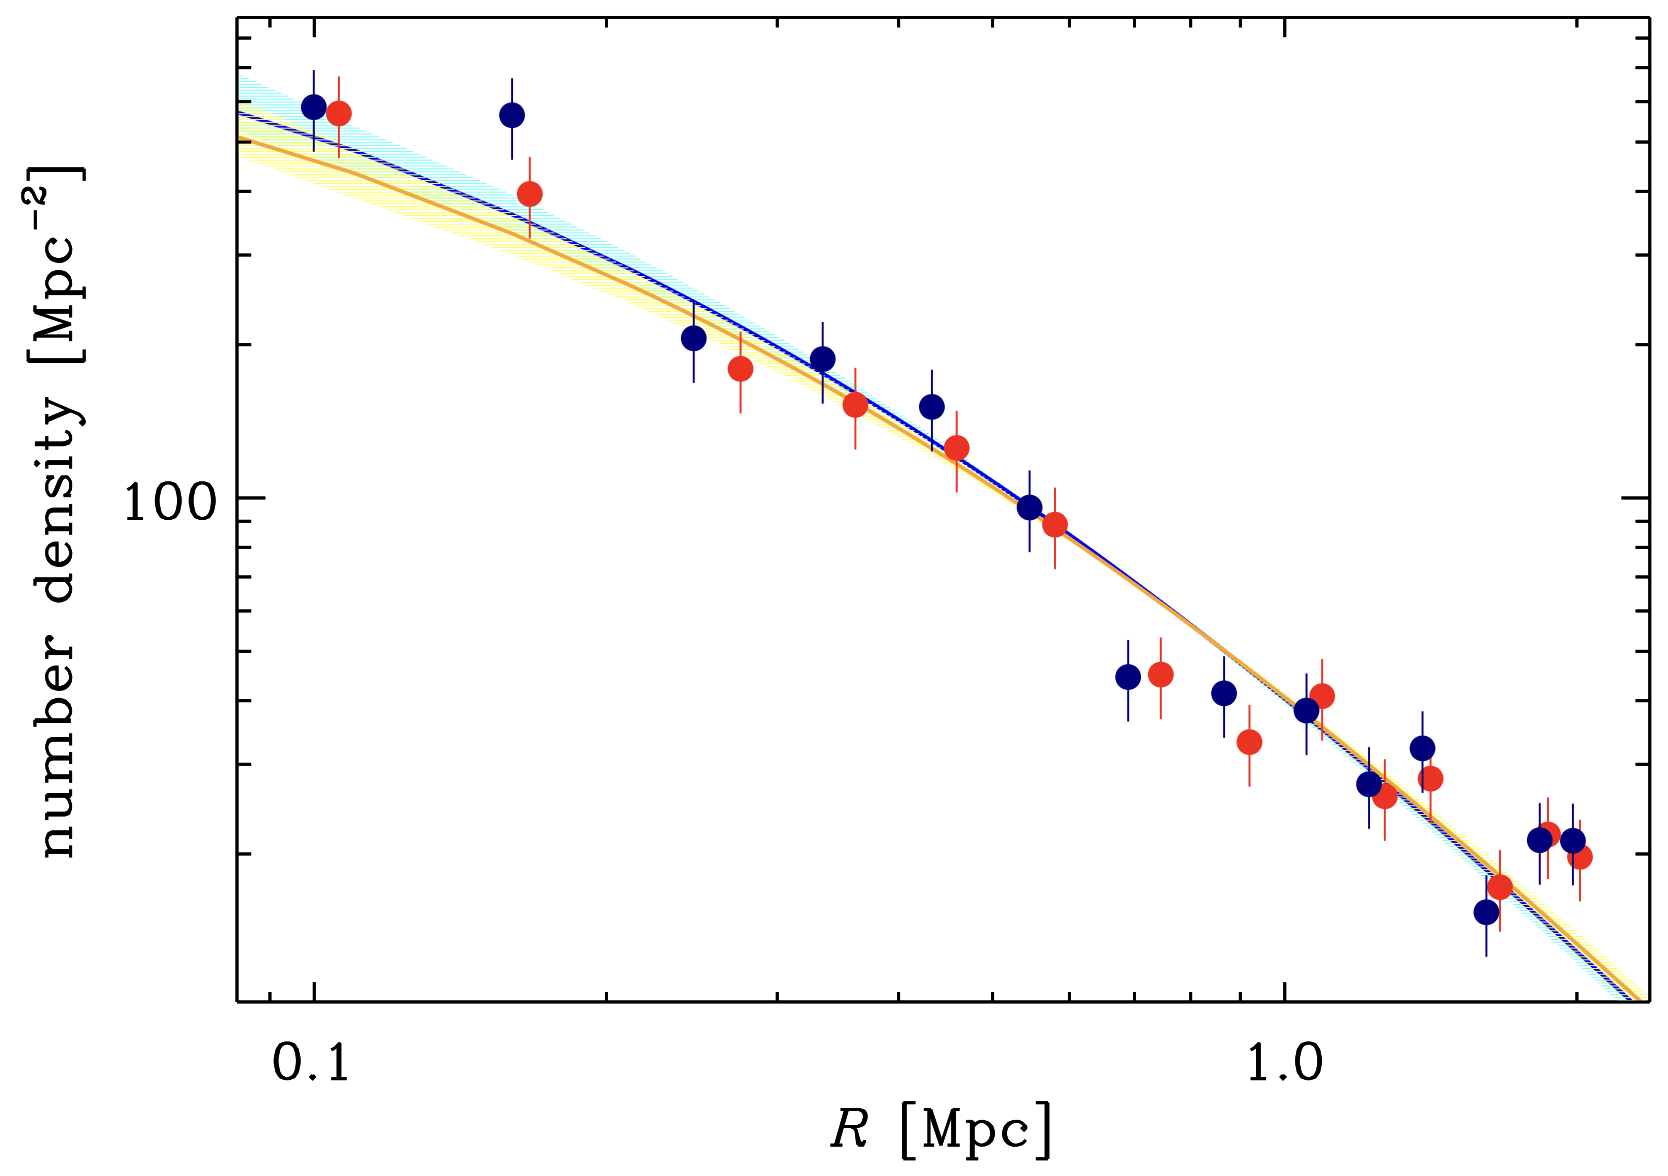
\includegraphics[width=0.6\linewidth]{Images/Chapter4/Number density MG-MAMPOSSt.png}
    \caption[Fit for number density density for MACS 1206]{Plot show projected number density profiles of cluster members. In particular, we are only interested in the CLUMPS selected members, marked with red dots. The orange line represents the best fit and the yellow area a confidence interval equal to 1$\sigma$. Figure 5 in ref. \cite{CLASH-VLT:-The-Inner-Slope-of-the-MACS-J1206.2-0847-Dark-Matter-Density-Profile}.}
    \label{fig:number density profile fit MACS 1206}
\end{figure}

The analytical expression for the dispersion of radial velocities can be found by integrating the Jeans equation \eqref{Equazione di Jeans sferica} and can be written as follows (ref. \cite{MG-MAMPOSST:a-code-to-test-modifications-of-gravity-with-internal-kinematics-and-lensing-analyses-of-galaxy-clusters}, \cite{Biviano_MAMPOSSt})
\begin{equation}
    \sigma^2 _r (r) = \frac{1}{\nu(r)} \int_r ^\infty \exp \qty(2\int_r ^s \frac{\beta(t)}{t} dt) \nu (s) \frac{d\Phi}{ds} ds,
\end{equation}
where the local velocity dispersion along the line of sight is 
\begin{equation}
    \sigma_z^2 (r, R) = \qty[1-\beta(r)\qty(\frac{R}{r})^2].
\end{equation}

Finally, the code output is the probability to observe a galaxy with position $R_i$ and velocity dispersion $v_{z,i}$ with $\theta$ that represents a set of parameters. In these terms, the output is the following:
\begin{equation}
    - \ln \mathcal{L} = -\sum_{i=1} ^N \ln q(R_i, v_{z,i} | \theta) ,
\end{equation}
where $\mathcal{L}$ is the likelihood, $N$ is the number of galaxies in the projected phase space, $\theta$ is a set of parameters and $q(R_i, v_{z,i})$ is the probability of observing a galaxy with projected position $R_i$ and l.o.s $v_{z,i}$. This probability is analytically written as
\begin{equation}
    q(R, v_z) = \frac{2 \pi R g(R, v_z)}{N_{\text{proj}} (R_{\text{max}}) - N_{\text{proj}} (R_{\text{min}})},
\end{equation}
where $N_{\text{proj}} (R)$ is the number of galaxies in the projected cylinder. Instead $g(R, v_z)$ is the surface density of the observed objects
\begin{equation}
    g(R, v_z) = \sqrt{\frac{2}{\pi}} \int_R ^\infty \frac{r\nu(r)}{\sigma_z (R, r) \sqrt{r^2 - R^2}} \text{exp}\qty(-\frac{v_z^2}{2\sigma_z^2(R, r)})dr.
\end{equation}
The version of the code we are using is equipped with a module to fit the velocity distribution of the BCG; this modifies the likelihood in the following form
\begin{equation}
    \mathcal{L}_{\text{kyn}} (\theta) = \mathcal{L}_{\textsc{MAMPOSSt}} (\theta) + \frac{\chi^2_{BCG} (\theta)}{2},
\end{equation}
where $\chi^2$ is the chi-square obtained between the theoretical prediction of $\sigma^2_{teo}$ and the observed data points $\sigma^2_{obs}$ of the BCG.

\section{Kinematic analysis of MACS 1206}
As we said in the previous chapter, we will study the cluster called MACS 1206 due to its physical properties; it performs well under the assumptions of spherical symmetry and dynamical relaxation.
The reconstruction of the mass profile occurs via a multi-component approach, in fact each component is modeled differently and the sum of the component provides the total mass of the cluster
\begin{equation}
    M_{\text{tot}} (r) = M_{\text{DM}} (r) + M_{\text{ICM}} (r) + M_{\text{BCG}} (r) + M_{*} (r),  
\end{equation}
where $M_{\text{DM}}$ stand for dark matter mass profile and it is modeled with a gNFW profile described in Chapter \ref{Dark matter properties}, the reason why we chose the gNFW and not the NFW is $\gamma$ dependence that provides information about the nature of dark matter. $M_{\text{BCG}}$ is the mass profile of the Brightest Cluster Galaxy which we modeled with a Jaffe profile \eqref{jaffe profile} and Jaffe's radius fixed at $r_J = 0.039$ Mpc.\\ For the ICM profile, we have adopted two different ways: in the first one we used a beta profile with a beta exponent equal to 1 and, in the second one we have previously fitted the gas data with a beta profile, obtaining the parameters that characterize the latter. In the end, for the other galaxies (excluding BCG) we adopted a pNFW profile. The result of this fit can be found in table \ref{tab:fit beta model}.

\begin{table}[h!]
    \centering
    \begin{tabular}{@{}lccc@{}}
        \toprule
        \textbf{Parameter} & \textbf{Value} & \textbf{Error (within 1$\sigma$)} & \textbf{Unit}\\
        \midrule
        $\rho_0$       & $4.51 \cdot 10^{14}$ & $4.12 \cdot 10^{12}$    & $M_\odot \; \text{Mpc}^{-3}$\\
        $r_c$          & $0.17$               & $0.17 \cdot 10^{-2}$     & Mpc\\
        $\alpha$       & $0.67$               & $0.23 \cdot 10^{-2}$     & - \\
        \bottomrule
    \end{tabular}
    \caption[Fit for $\beta$ profile]{Fit for $\beta$ profile, note that $\beta$ is almost 2/3.}
    \label{tab:fit beta model}
\end{table}



Before the analysis, we have to set some cosmological parameters; in particular, the following fixed values are used: $H_0 = 70 \; \text{km} \; \text{s}^{-1} \; \text{Mpc}^{-1}$ at $z = 0$, the redshift of the cluster $z = 0.4398$, the matter density $\Omega_m = 0.3$ and dark energy density $\Omega_\Lambda = 0.7$.\\
These parameters remain constant and the same for each run of the code.\\
In order to eliminate any interlopes in our sample, a specific method is developed according to ref. \cite{CLASH-VLT:-The-Inner-Slope-of-the-MACS-J1206.2-0847-Dark-Matter-Density-Profile}. CLUster Membership in Phase Space (or CLUMPS) is based on the determination of peaks in the velocity distribution of galaxies in function of the clustercentric distance (distance from the center of the cluster). In the end, velocity boundaries are defined thanks to the minimum around the velocity peak and interlopers are removed (see ref. \cite{Biviano_CLUMPS} for more details).\\ Other methods are also developed such as P+G and CLEAN but they are not used in this thesis.\\
The sample includes 468 galaxies (tracers), and 463 were used by the code to fit in a radial range between 0.055 Mpc and 2.153 Mpc in MCMC mode with an MCMC sample 110\,000 points in the parameter space.\\
\begin{figure}[h!]
    \centering
    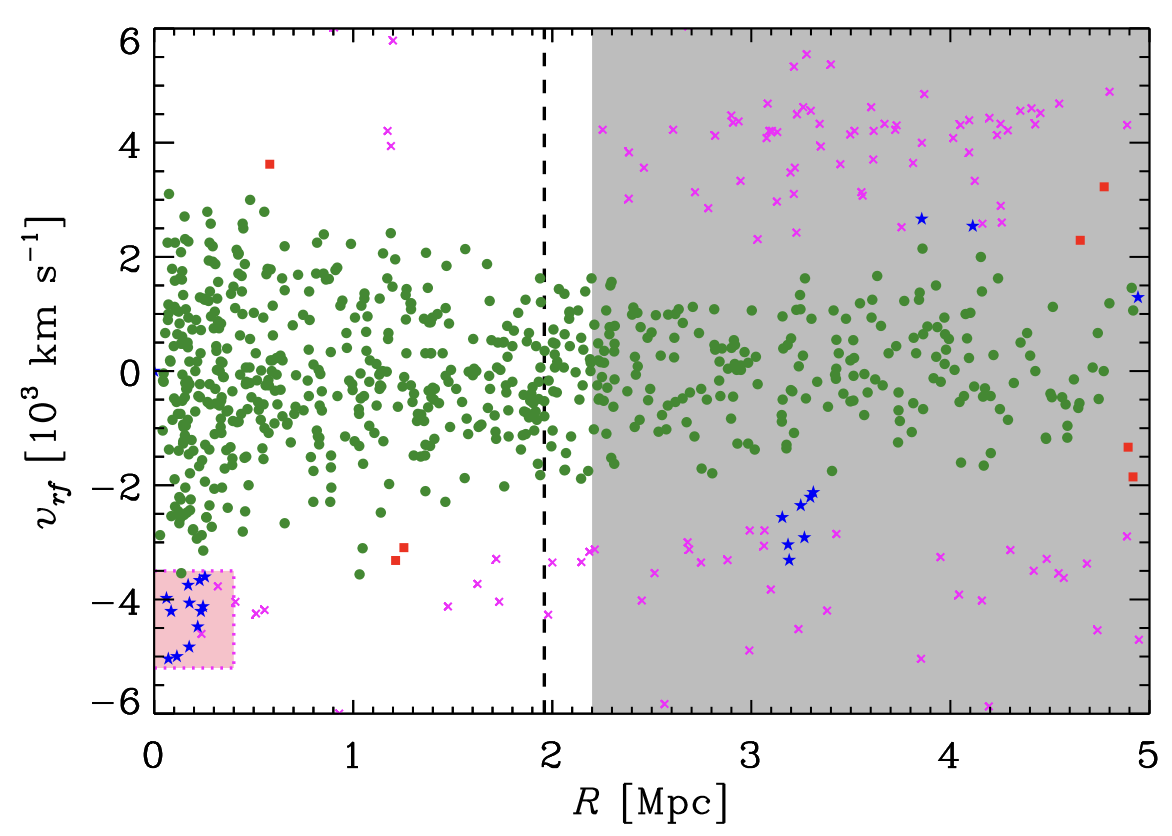
\includegraphics[width=0.6\linewidth]{Images/Chapter4/projected space phase.png}
    \caption[Projected space phase for MACS 1206]{Projected space phase for MACS 1206, the pink enta area indicates galaxies that are not selected as members. The vertical dashed line indicates the virial radius. The gray area has not been considered as it is located at radii greater than 2.2 Mpc. The red squared are members selected by CLUMPS, blue stars are selected by P+G, green dots indicate members selected by CLUMPS and P+G. In Finally, magenta stars indicate members not selected by these two methods. Figure 1 in ref. \cite{CLASH-VLT:-The-Inner-Slope-of-the-MACS-J1206.2-0847-Dark-Matter-Density-Profile}.}
    \label{fig:projected space phase}
\end{figure}\\

Furthermore, it is important to say that different velocity anisotropy models were used for BCG and for the rest of the cluster; in fact, for BCG we choose an Osipkov-Merritt, or more simply "OM" (ref. \cite{Osipkov_1979}, \cite{Merritt_1985}) and follow this analytical distribution
\begin{equation}
    \beta_{BCG} (r) = \frac{r^2}{r^2 + r^2_a},
\end{equation}
where $r_a$ is the scale radius set to 20 Mpc. With this value, the OM profile is almost constant in the entire range.\\ Instead, for the anisotropy model of the rest of the cluster, we adopted two different profiles in order to find the best. The gT anisotropy profile \eqref{gT model} and BP profile \eqref{BP model} which we introduced previously.\\
In \textsc{MG-MAMPOSSt}, the velocity anisotropy of member galaxies is actually defined in terms of the rescaled parameters $\mathcal{A}_0$ and $\mathcal{A}_\infty$ through the relation $\mathcal{A}_0 = (\sigma_r/\sigma_\theta)_0 = (1-\beta_0)^{-1/2}$ and similarly $\mathcal{A}_\infty = (\sigma_r/\sigma_\theta)_\infty = (1-\beta_\infty)^{-1/2}$.\\

Overall, the analysis consists of 4 \textsc{MG-MAMPOSSt} runs: in the first, a gT type model is used for the anisotropy, leaving the $r_\beta$ parameter free; in the second run, the same procedure is performed with a BP type model for the anisotropy; a third run employs a BP model for the anisotropy with $r_\beta$ fixed; in particular we decided to set $r_\beta = 1 \; \text{Mpc}$ because Mpc is the typical dimension for a cluster galaxy. Instead, the last run was performed with a BP anisotropy model but a different beta profile because the exponent  $\beta$ in profile \eqref{gas fit} was set equal to 2/3 instead of equal to one as in the first three mentioned above.\\


So we have a total of 8 free parameters listed in the following table, together with the lower and upper limits imposed through flat priors.
\begin{table}[h!]
    \centering
    \begin{tabular}{@{}lccc@{}}
        \toprule
        \textbf{Parameter} & \textbf{Lower limit} & \textbf{Upper limit} & \textbf{Unit}\\
        \midrule
        $r_{200}$                      & 0.50 & 5.00 & Mpc\\
        $r_{\nu}$ (tracer scale)           & 0.39 & 0.54 & Mpc\\
        $r_{s}$                      & 0.04 & 3.90 & Mpc\\
        $\mathcal{A}_\infty$ (anisotropy, outer)  & 0.30 & 5.10 & -\\
        $\mathcal{A}_0$ (anisotropy, central)     & 0.50 & 4.10 & -\\
        $X_L$      & 2.01 & 7.00 & $M_\odot/L_\odot$\\
        $\gamma$ (gNFW inner slope)               & 0.30 & 2.00 & -\\
        $r_{\beta}$                         & 0.03 & 3.10 & Mpc\\
        \bottomrule
    \end{tabular}
    \caption[Free parameters and relative bounds for \textsc{MG-MAMPOSSt} analysis]{The 8 free parameters with their lower and upper limits and their units.}
    \label{tab:8 free parameter in gT with beta free run}
\end{table}


\section{Results}

The results of the four scenarios discussed above are listed in table \ref{results}, where we list the constraints on the parameters at 2$\sigma$.

\begin{table}[h!]
    \centering
    \begin{threeparttable}
    \resizebox{1.0\textwidth}{!}{
    \begin{tabular}{l|cccccccc}
        \toprule
        \Large $\beta$ model & \Large $r_{200}$ [Mpc] & \Large $r_{\nu}$ [Mpc] & \Large $r_s$ [Mpc] & \Large $\mathcal{A}_\infty$ & \Large \textbf{$\gamma$} & \Large $\mathcal{A}_0$ & \Large $r_\beta$ [Mpc] & \Large $X_L$ [M$_\odot$/L$_\odot$]\\
        \midrule
        \Large gT ($r_\beta$ free)  & \Large $2.02^{+0.20}_{-0.18}$ & \Large $0.41^{+0.04}_{-0.02}$ & \Large $0.53^{+0.32}_{-0.22}$ & \Large $2.75^{+1.96}_{-1.39}$ & \Large $0.57^{+0.28}_{-0.26}$ & \Large $1.28^{+1.16}_{-0.87}$ & \Large $0.42^{+1.46}_{-0.45}$ & \Large $4.46^{+0.21}_{-0.23}$ \\ [0.3cm]
        %\addlinespace[11pt]
        \Large BP ($r_\beta$ free)  & \Large $2.03^{+0.20}_{-0.19}$ & \Large $0.41^{+0.03}_{-0.02}$ & \Large $0.54^{+0.36}_{-0.24}$ & \Large $2.70^{+2.00}_{-1.53}$ & \Large $0.57^{+0.29}_{-0.26}$ & \Large $1.07^{+1.06}_{-0.62}$ & \Large $0.37^{+2.25}_{-0.48}$ & \Large $4.46^{+0.22}_{-0.23}$ \\ [0.3cm]
        %\addlinespace[11pt]
        \Large BP ($r_\beta$ fixed) & \Large $2.02^{+0.23}_{-0.21}$ & \Large $0.41^{+0.03}_{-0.02}$ & \Large $0.51^{+0.70}_{-0.23}$ & \Large $2.62^{+2.12}_{-1.47}$ & \Large $0.51^{+0.37}_{-0.22}$ & \Large $1.20^{+0.73}_{-0.42}$ & \Large -- & \Large $4.48^{+0.22}_{-0.25}$ \\ [0.3cm]
        %\addlinespace[11pt]
        \Large BP ($r_\beta$ free)$^{\ast}$ & \Large $1.96^{+0.33}_{-0.36}$ & \Large $0.41^{+0.04}_{-0.02}$ & \Large $0.46^{+0.35}_{-0.27}$ & \Large $2.85^{+1.90}_{-1.57}$ & \Large $0.47^{+0.39}_{-0.40}$ & \Large $1.01^{+0.89}_{-0.59}$ & \Large $0.40^{+2.32}_{-0.40}$ & \Large $4.50^{+0.26}_{-0.27}$ \\
        \bottomrule
    \end{tabular}
    }
    \caption[Results of analyses with \textsc{MG-MAMPOSSt} for MACS 1206]{Results of the four runs performed with BP and gT anisotropy models. For each parameter the median and the 95\% credible interval are reported. In the case of BP with fixed $r_\beta$, the transition radius is not a free parameter.}
    \label{results}
    \begin{tablenotes}
        \small
        \item[$^{\ast}$] This run also includes the fit of the gas component.
    \end{tablenotes}
    \end{threeparttable}
\end{table}

From the results in table \ref{results}, it is possible to notice that, with the same number of free parameters, the gT model and the BP model give substantially identical results for $\gamma$.\\ To qualitatively determine which was better among the runs with the BP pattern (one with and the other without free $r_\beta$), we use the Bayesian Information Criterion (BIC hereafter) defined as follows
\begin{equation}
    \text{BIC} = k\ln{n} - 2\ln{\mathcal{L}},
\end{equation}
where $k$ is the number of parameters, $n$ the size of sample and $\mathcal{L}$ the likelihood value. In this case all samples were composed, as said before, from 463 explored galaxies. The code returns the $-\ln{\mathcal{L}}$ and it is therefore easy to check that the BP model with $r_\beta$ free is favored thanks to a BIC $=$ 8628.14 against a BIC $=$ 8633.84 for the fixed $r_\beta$. You consequently have a $\Delta$BIC $=$ 5.70.\\
We therefore decided to focus on the BP model with free $r_\beta$ which, from the BIC value, proved to be the most promising model.\\
$r_{200}$ represents the virial radius of dark matter halo, defined as the distance from the center within which the average density of the dark matter halo is 200 times the critical density of the universe. For MACS 1206, this radius is about 2 Mpc in every analysis. Physically, $r_{200}$ bounds the gravitationally bound region of the cluster and provides a scale of magnitude: outside this radius, the density drops below 200 times the critical density, and the material is no longer tightly bound to the cluster.\\
$r_{\nu}$ is the scale radius of the radial distribution of galaxies that are members of the cluster. In this case $r_{\nu}$ is smaller than $r_{200}$, so that means that galaxies are distributed in a more concentrated way than dark matter and, in particular, closer to the center of the cluster.\\
$r_s$ is the scale radius of the gNFW profile and represents the scale beyond which the density profile begins to decline most rapidly.\\
As it concerns $r_\beta$, the transition radius of the anisotropy, it is possible to notice how the latter is very close to zero, this indicates an almost constant anisotropy from the center of the cluster to the outermost regions. More generally, this was found to be true for both the gT model and the BP model.\\
Focusing instead on the $\gamma$ parameter of the gNFW, our main object of interest, we obtain e.g. $\gamma = 0.57^{+0.29}_{-0.26}$ for the BP-$r_\beta$-free model, lower than the value found in ref. \cite{CLASH-VLT:-The-Inner-Slope-of-the-MACS-J1206.2-0847-Dark-Matter-Density-Profile}. This is valid in all the tested scenarios.\\ We recall here that $\gamma$ describes the internal slope of the dark matter density profile in the cluster.
In case of a pure NFW we have $\gamma=1$ but a smaller value indicates a density towards the center that grows flatter, creating a less cuspidate profile and more cores.\\
When further changing the fit to the gas mass data in the fourth run of Table \ref{tab:8 free parameter in gT with beta free run} (where we used $\beta = 2/3$ in \eqref{gas fit}\footnote{Note that here, the $\beta$ parameter is the exponent used in the radial distribution for gas.}, providing a better fit with respect to the case $\beta=1$) we obtain an even lower value.
This is extremely important because, as we discussed before, $\gamma$ may be indicative about the type and interaction of dark matter, bringing also information of any possible baryonic feedback.
Coming back to $\gamma$, this is lower but still within the limits of a slope generated by cold dark matter within the standard cosmological model.\\
Also, from the figure \ref{fig:distribuzioni marginali dei parametri modello BP e freebeta_1} it is possible to see how $X_L$  tends to follow a trend opposite to $\gamma$, as the mass/brightness ratio increases the $\gamma$ parameter decreases and vice versa. This remains valid in all regimes used, both gT and BP. Consequently, this seems to indicate that a greater presence of baryonic mass tends to make the dark matter slope less steep.

\begin{figure}[h!]
    \centering
    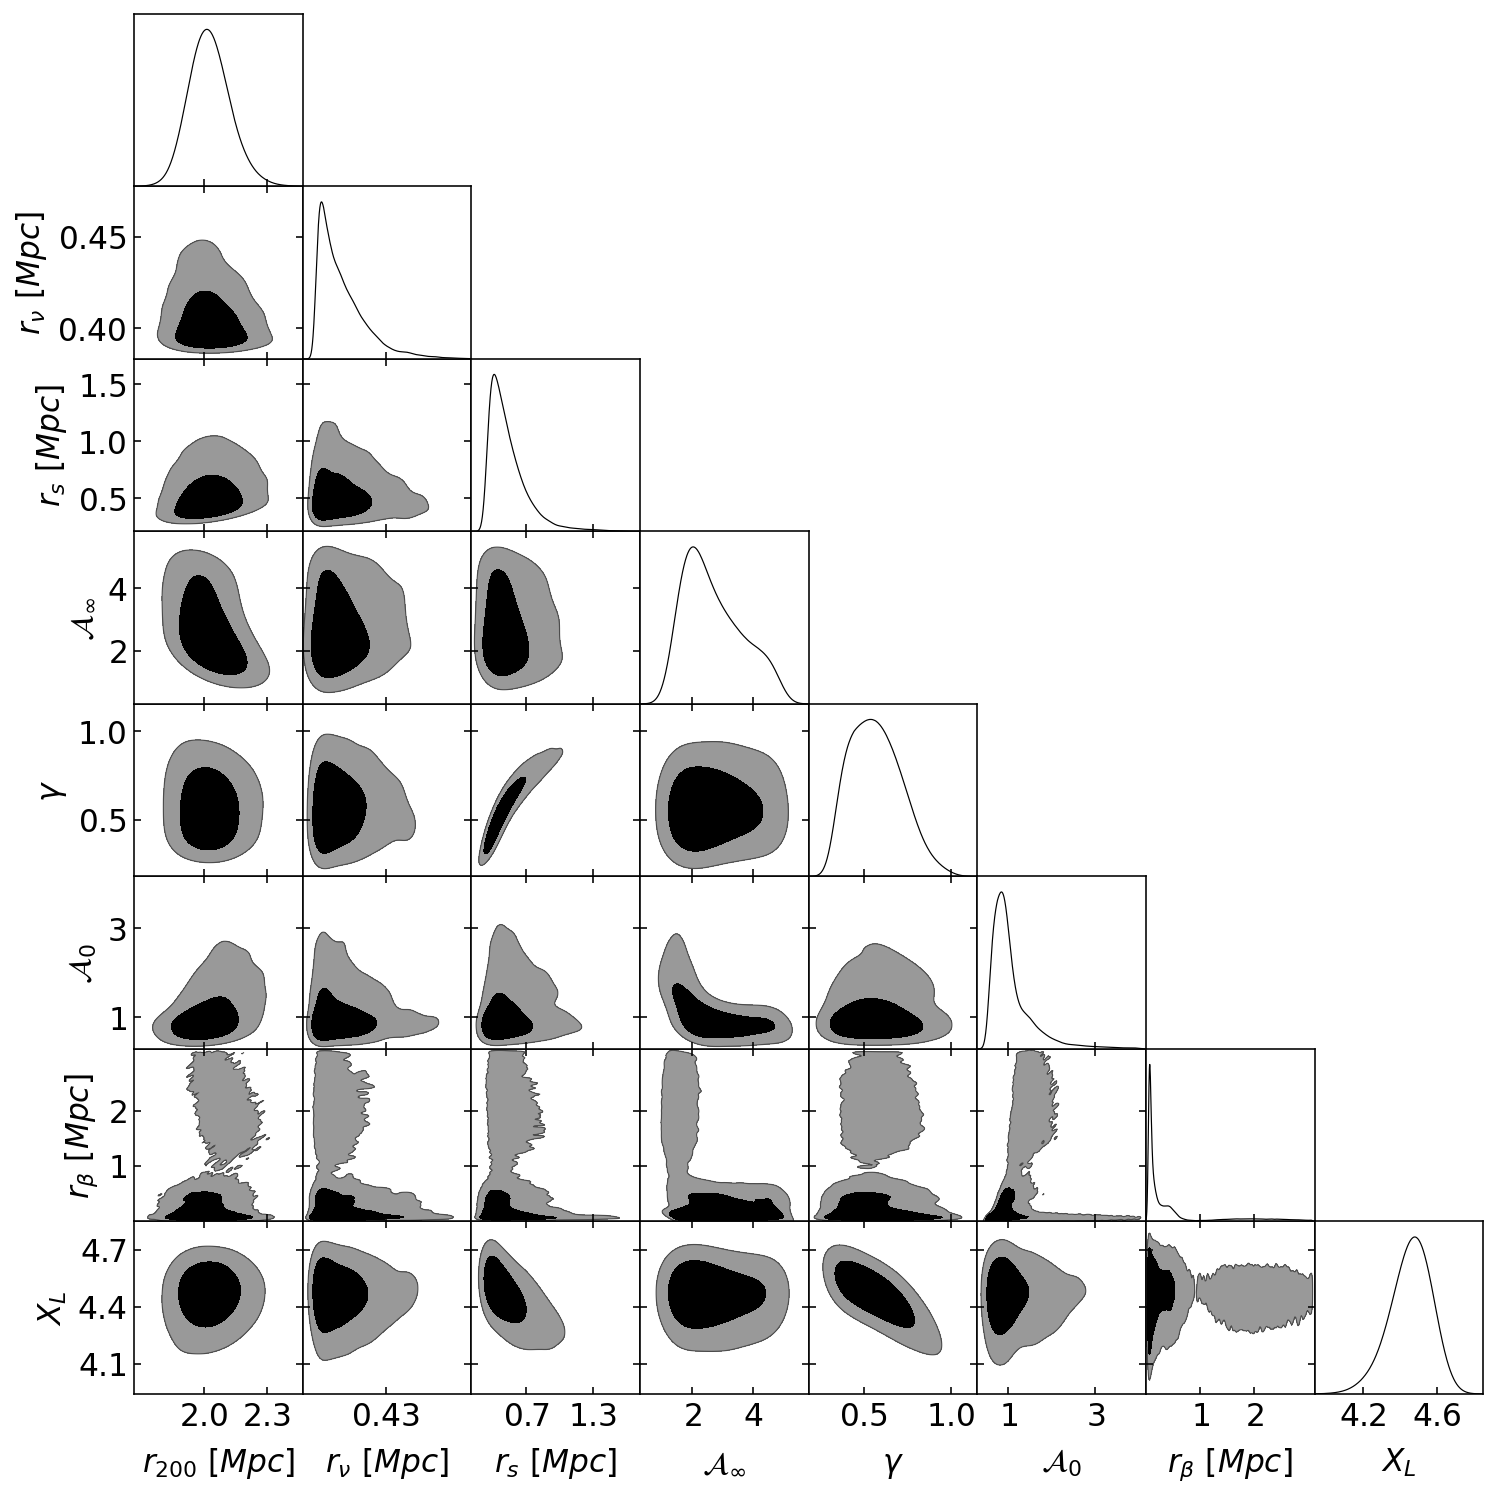
\includegraphics[width=0.9\linewidth]{Images/Chapter4/BP freebeta=1/distribution BP freebeta=1.png}
    \caption[Marginal distributions of parameters in the BP model with free $r_\beta$]{Marginal distributions of parameters in the BP model with free $r_\beta$. The darker region indicates the uncertainty interval equal to 1$\sigma$ (68\;\%) and the gray zone an uncertainty interval equal to 2$\sigma$ (95\;\%).}
    \label{fig:distribuzioni marginali dei parametri modello BP e freebeta_1}
\end{figure}

\clearpage

\subsubsection{Decomposition of mass}
In fig. \ref{fig:decomposione della massa modello BP e freebeta_1} the total kinematic mass distribution obtained with \textsc{MG-MAMPOSSt} is reported. The plot shows how, at very small radii, the BCG contribution dominates, only to be overtaken by dark matter while BCG mass becomes constant. This is expected because BCG has a radius measured in kpc. It's also important to note that although the contribution of galaxies, and especially gas, increases considerably, dark matter remains predominant all the way to the outermost regions, almost matching the cluster's overall mass profile. This behavior is completely analogous in every run conducted, thus underlining the importance of dark matter and how this is actually the main component of the cluster.

\begin{figure}[h!]
    \centering
    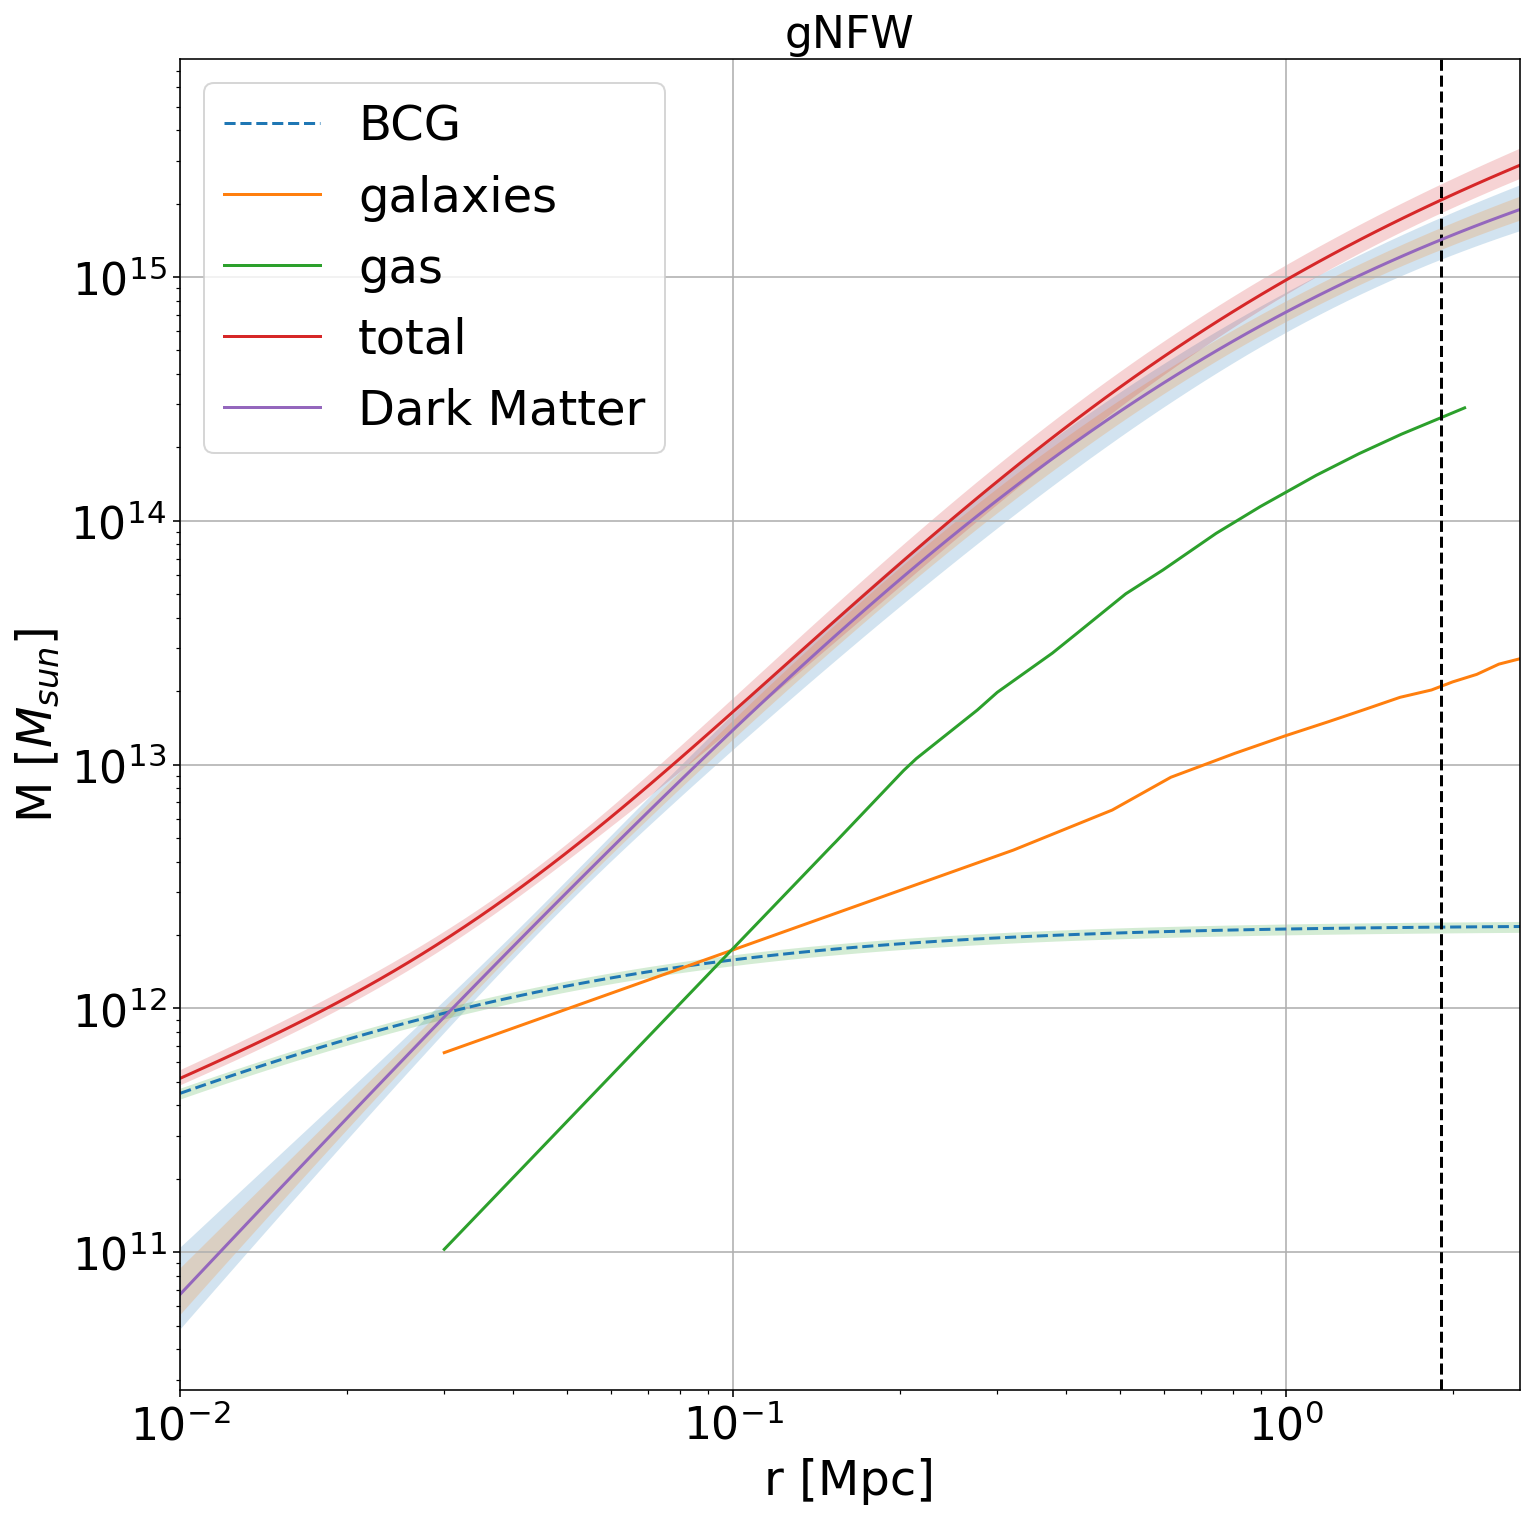
\includegraphics[width=0.50\linewidth]{Images/Chapter4/BP freebeta=1/mass reconstruction BP freebeta=1.png}
    \caption[Mass decomposition with BP model and free $r_\beta$]{Mass decomposition with BP model and free $r_\beta$. The dashed vertical line represents the upper limit of the radial range used for the fit, with a value equal to 2.153 Mpc.}
    \label{fig:decomposione della massa modello BP e freebeta_1}
\end{figure}


\subsubsection{Anisotropy profile}

In fig. \ref{fig:anisotropy_profiles} we can see the anisotropy profile for the first three runs described above. The reconstruction of $\beta(r)$ shows moderately radial orbits already at the center and a growth towards more radial values as the radius increases. The black curve in fact starts around $\beta \sim 0.4$ and tends asymptotically to $\beta \sim 0.75$ beyond 1 Mpc. Here too, the confidence bands are indicated with a darker color within 1 $\sigma$ and lighter within 2$\sigma$.\\
$\mathcal{A}_0$ is related to central anisotropy, that is, how the velocities of galaxies near the center of the cluster are oriented. From the plot you can see how in the gT model the anisotropy for $r \rightarrow 0$ is $\sim 0.4$, compatible with a weak radial anisotropy. This means that, near nucleus, galaxies move with very similar speeds in all directions.\\
$\mathcal{A}_\infty$ is related to anisotropy at large distances and $\beta$ grows indicating markedly radial orbits towards the peripheries of the cluster.\\ In the BP model, with and without $r_\beta$ fixed, $\beta$ start from $\sim$ 0.25, which indicate more isotropic orbits where the radial and tangential directions are equivalent.\\
It’s interesting to note the bump in the anisotropy profile in the BP template with $r_\beta$ fixed (center plot). This result does not have a strictly physical nature; it is due to the rigidity on the position of the transition from $\beta_0$ to $\beta_\infty$. In fact, forcing the transition to a fixed radius, fit introduce a local curvature to better adapt velocity dispersions. This is demonstrated precisely by the plot of the BP model but having a free $r_\beta$ (right plot), in this case the bump is significantly reduced.
Finally, the gT model instead adopts a softer profile which, thanks to a free beam, completely eliminates this bump (left plot).

\begin{figure}[h!]
    \centering
    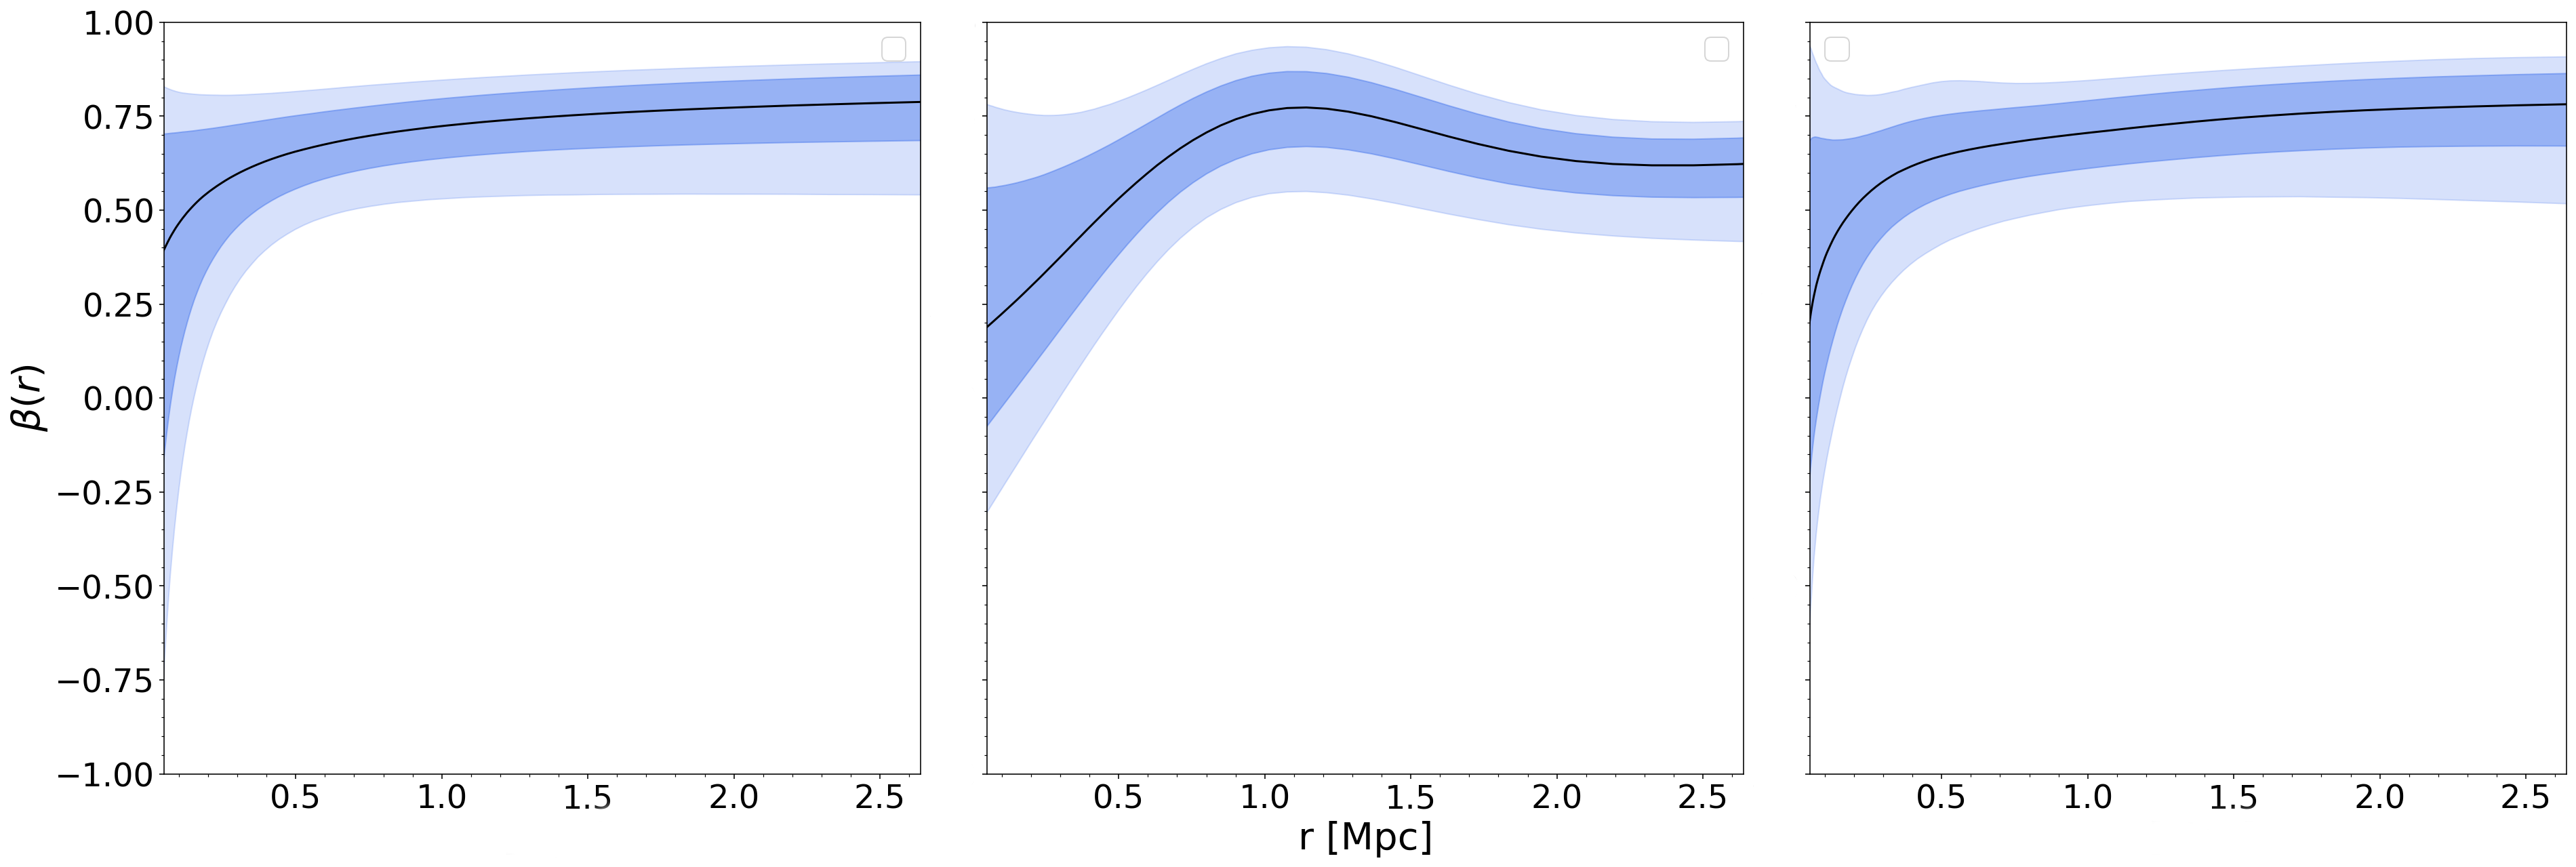
\includegraphics[width=1.0\linewidth]{Images/Chapter4/anisotropia.png}
    \caption[Comparison between anisotropy profile for each anisotropy model and $r_\beta$]{
    \textbf{Left panel}: anisotropy profile for gT model and free $r_\beta$. 
    \textbf{Center panel}: BP model with fixed $r_\beta$, showing a clear bump in the anisotropy profile. 
    \textbf{Right panel}: BP model with free $r_\beta$, with a smaller bump around $r \sim 0.5$ Mpc. 
    In each panel, the darker region corresponds to $1\sigma$ uncertainty, and the lighter to $2\sigma$.
    }
    \label{fig:anisotropy_profiles}
\end{figure}